El perceptrón multicapa, también conocido como red neuronal de múltiples capas es un ejemplo de red neuronal profunda feedforward, es una extensión del perceptrón simple que consta de múltiples capas de neuronas interconectadas ver Figura \ref{fig:an7}. A diferencia del perceptrón de una sola capa, el perceptrón multicapa tiene al menos una capa oculta (capas entre la capa de entrada y la capa de salida), lo que le permite resolver problemas más complejos y no linealmente separables.

Esta red neuronal se entrena utilizando algoritmos de aprendizaje supervisado, como retropropagación (backpropagation), que ajustan los pesos de las conexiones entre las neuronas para minimizar una función de pérdida, mejorando así la capacidad de la red para hacer predicciones precisas.

\begin{figure}
	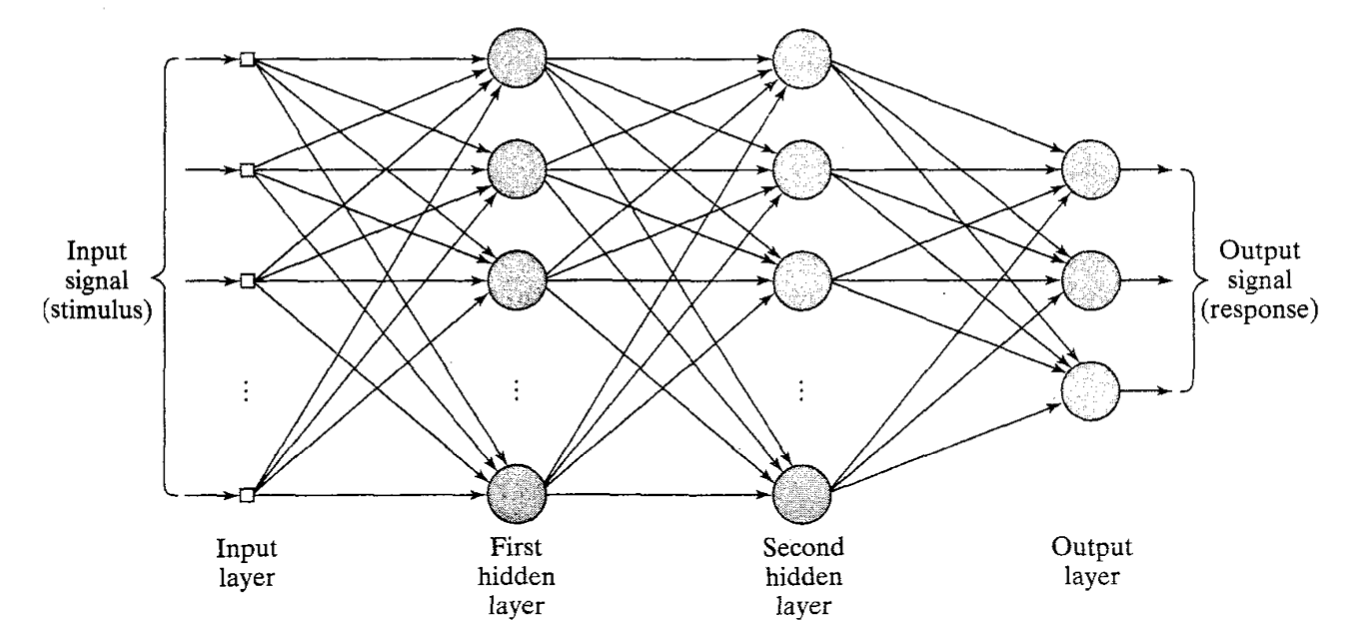
\includegraphics[width=0.65\textwidth]{capitulo2/figuras/an7.png}
	\caption{Grafo arquitectonico de un perceptron multicapa con dos capas ocultas}
	\floatfoot{Fuente: Neural networks: a comprehensive foundation \cite[p.281]{haykin1998neural}}
	\label{fig:an7}
\end{figure}

El perceptrón multicapa es una red neuronal típica, puede constar de varias capas y conexiones entre neuronas. En su arquitectura se observa la estructura básica de una red neuronal ver Figura \ref{fig:an7}, una de las arquitecturas más comunes que consta de: 
\begin{itemize}

	\item Capa de Entrada: 
	
	Esta capa recibe los datos brutos o características de entrada. Cada neurona en esta capa representa una característica o variable de entrada.

	\item Capas Ocultas: 
	
	Las capas ocultas (una o varias) entre la capa de entrada y la capa de salida procesan los datos y extraen características significativas de manera no lineal. Cada neurona en una capa oculta toma las salidas de la capa anterior como entrada, realiza cálculos y transfiere la salida a la siguiente capa.

	\item Capa de Salida:
	
	Esta capa produce la salida final de la red neuronal. La cantidad de neuronas en esta capa depende del tipo de problema que se esté abordando. Por ejemplo, en un problema de clasificación binaria, podría tener una neurona que produzca una salida entre 0 y 1. En problemas de clasificación multiclase, habría tantas neuronas de salida como clases a predecir, cada una representando la probabilidad de pertenencia a esa clase.
\end{itemize}